% !TEX root = ../main.tex

\section*{Gas state and pressure}

A basic theoretical study of the gas state and pressure inside the tanks has been conducted. To do so, the properties of the $N_2O$ have been extracted from \cite{n2oReference}. With the equations presented on the former source, a simple Matlab code has been built that generate the chart in Figure \ref{fig:N2O_P_V_graph}, said code can be found in \cite{MatlabPVchart}.

It's important to realize that its difficult to measure the amount of nitrous oxide remaining in the tank because the pressure inside the tank remains constant until the tank is almost empty. The reason why this happens is because inside the tank there is $N_2O$ in both vapor and liquid states. When this happens the pressure inside the tank remains constant at a value named vapor pressure.

This state where the two phases co-exist can only happen at a given pressure temperature and specific volume of the substance. A graphic representing this can be seen on the figure \ref{fig:N2O_P_V_graph}.

\begin{figure}[h]
  \centering
  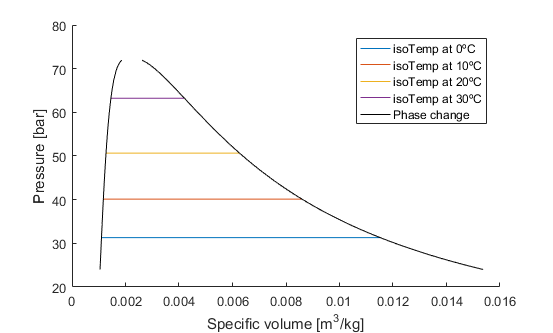
\includegraphics[width=0.8\textwidth]{N2O_pressure_volume.png}
  \caption{P vs v chart of $N_2O$}
  \label{fig:N2O_P_V_graph}
\end{figure}

The tank currently used to supply the gas is 5L and stored 3.75Kg of gas when it was full. That is $(0.005 m^3) / (3.75 kg)$ = $0.00133 m^3/kg$. Looking at the previous chart it's possible to see that this point was at the limit of the vapor-liquid zone and thus the tank was probably full of liquid at atmospheric temperature. However, this tank has already been used once and it's estimated that one-fourth of the content is gone. Then, the current specific volume is $(0.005 m^3) / (2.625 kg)$ = $0.0019 m^3/kg$. This value ensures that the substance will remain at vapor-liquid phase at any reasonable temperature.

When the rocket engine is connected to the gas tank and the valves are open, the pressure and the specific volume stabilize between the two recipients; this fills the engine integrated tank with liquid and vapor nitrous oxide.

The previous graph also shows the vapor pressure of the gas at different temperatures. It's important to notice the difference in pressure between common atmospheric temperatures. The current loading system has been prepared to withstand up to 70 bars plus security margins. This means that the launch or test ignition should be delayed if the temperatures are superior to 34.7ºC.

However, it must be noted, that thanks to the security margins and the fact that the gas colds down when expanded, the system would probably withstand a launch at more than this ambient temperature. All the same, security is a top priority and ANY LAUNCH WILL BE DELAYED if it's not possible to assure a tank temperature lower that.